\section{背景介绍}
\begin{frame}{地震波探测}
    \begin{figure}[ht]
        \centering
        \subfigure[共中点道集]{
            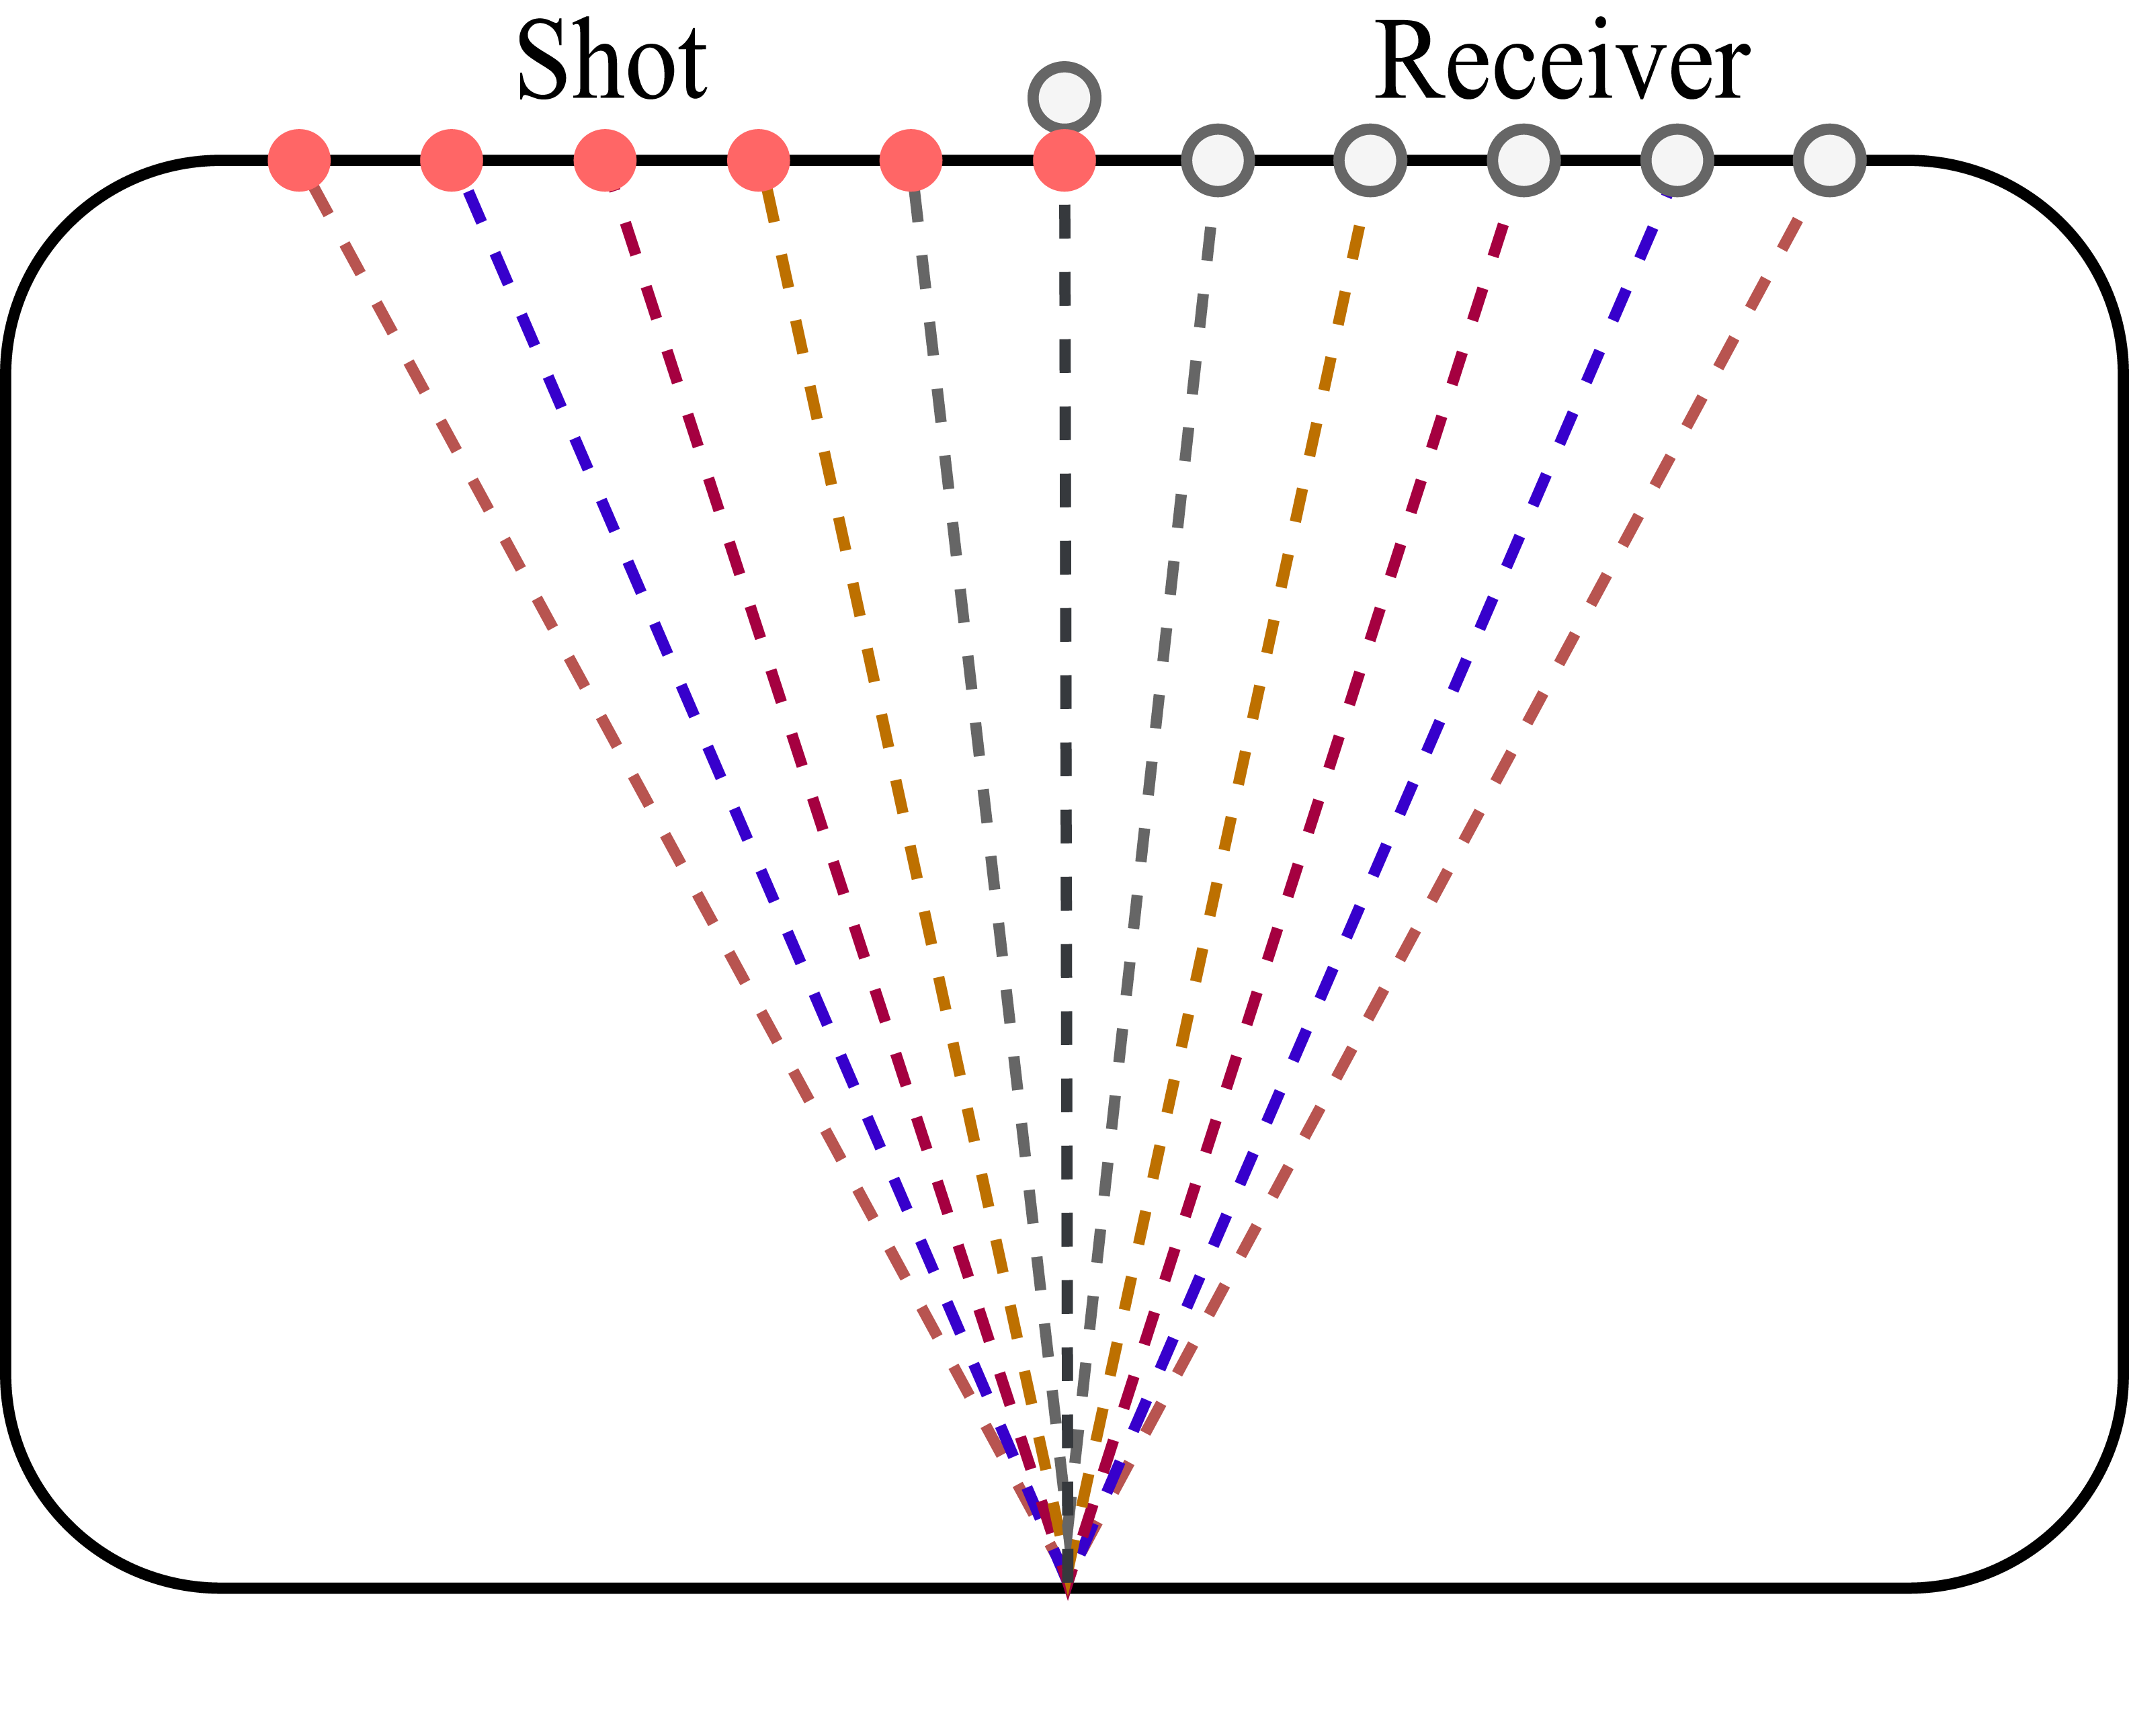
\includegraphics[height=4cm]{03_共中点道集.png}
        }\ 
        \subfigure[旅行时与偏移距的关系]{
            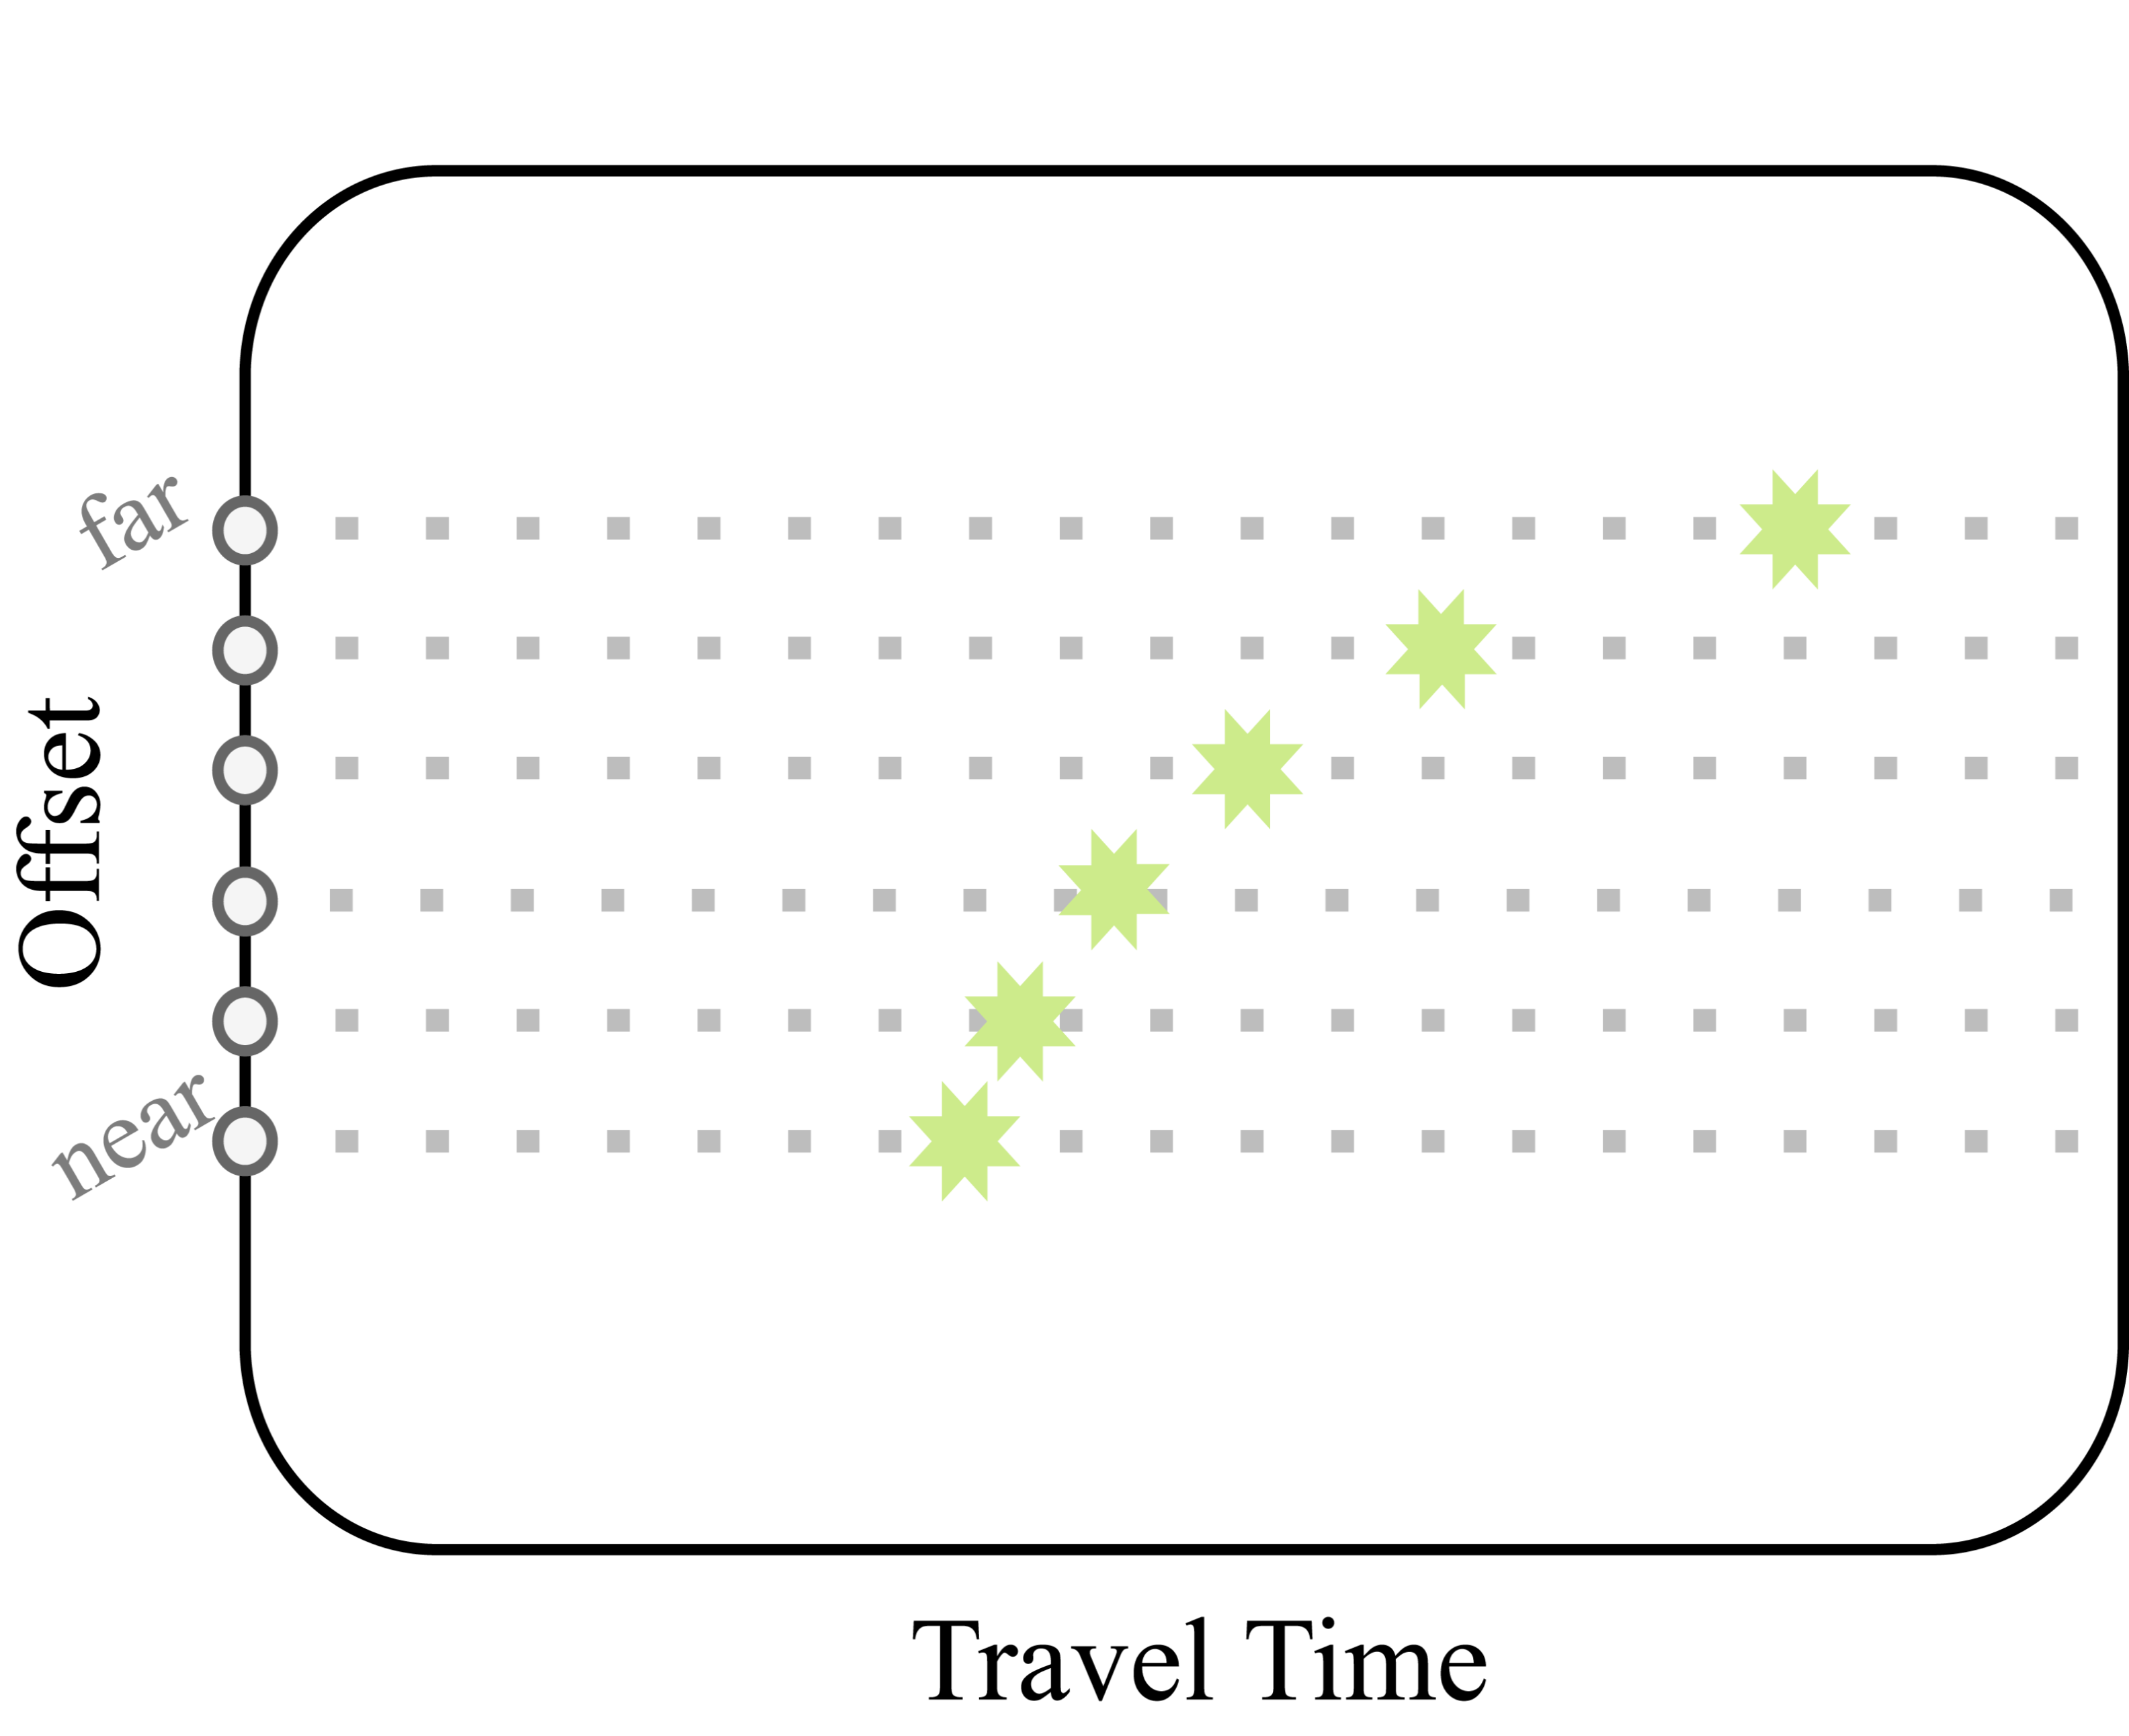
\includegraphics[height=4cm]{04_偏移距与旅行时图像_NMO前_copy.png}
        }
    \end{figure}
\end{frame} 

\begin{frame}{动校正}
    \begin{figure}[ht]
        \centering
        \subfigure[NMO前旅行时与偏移距的关系]{
            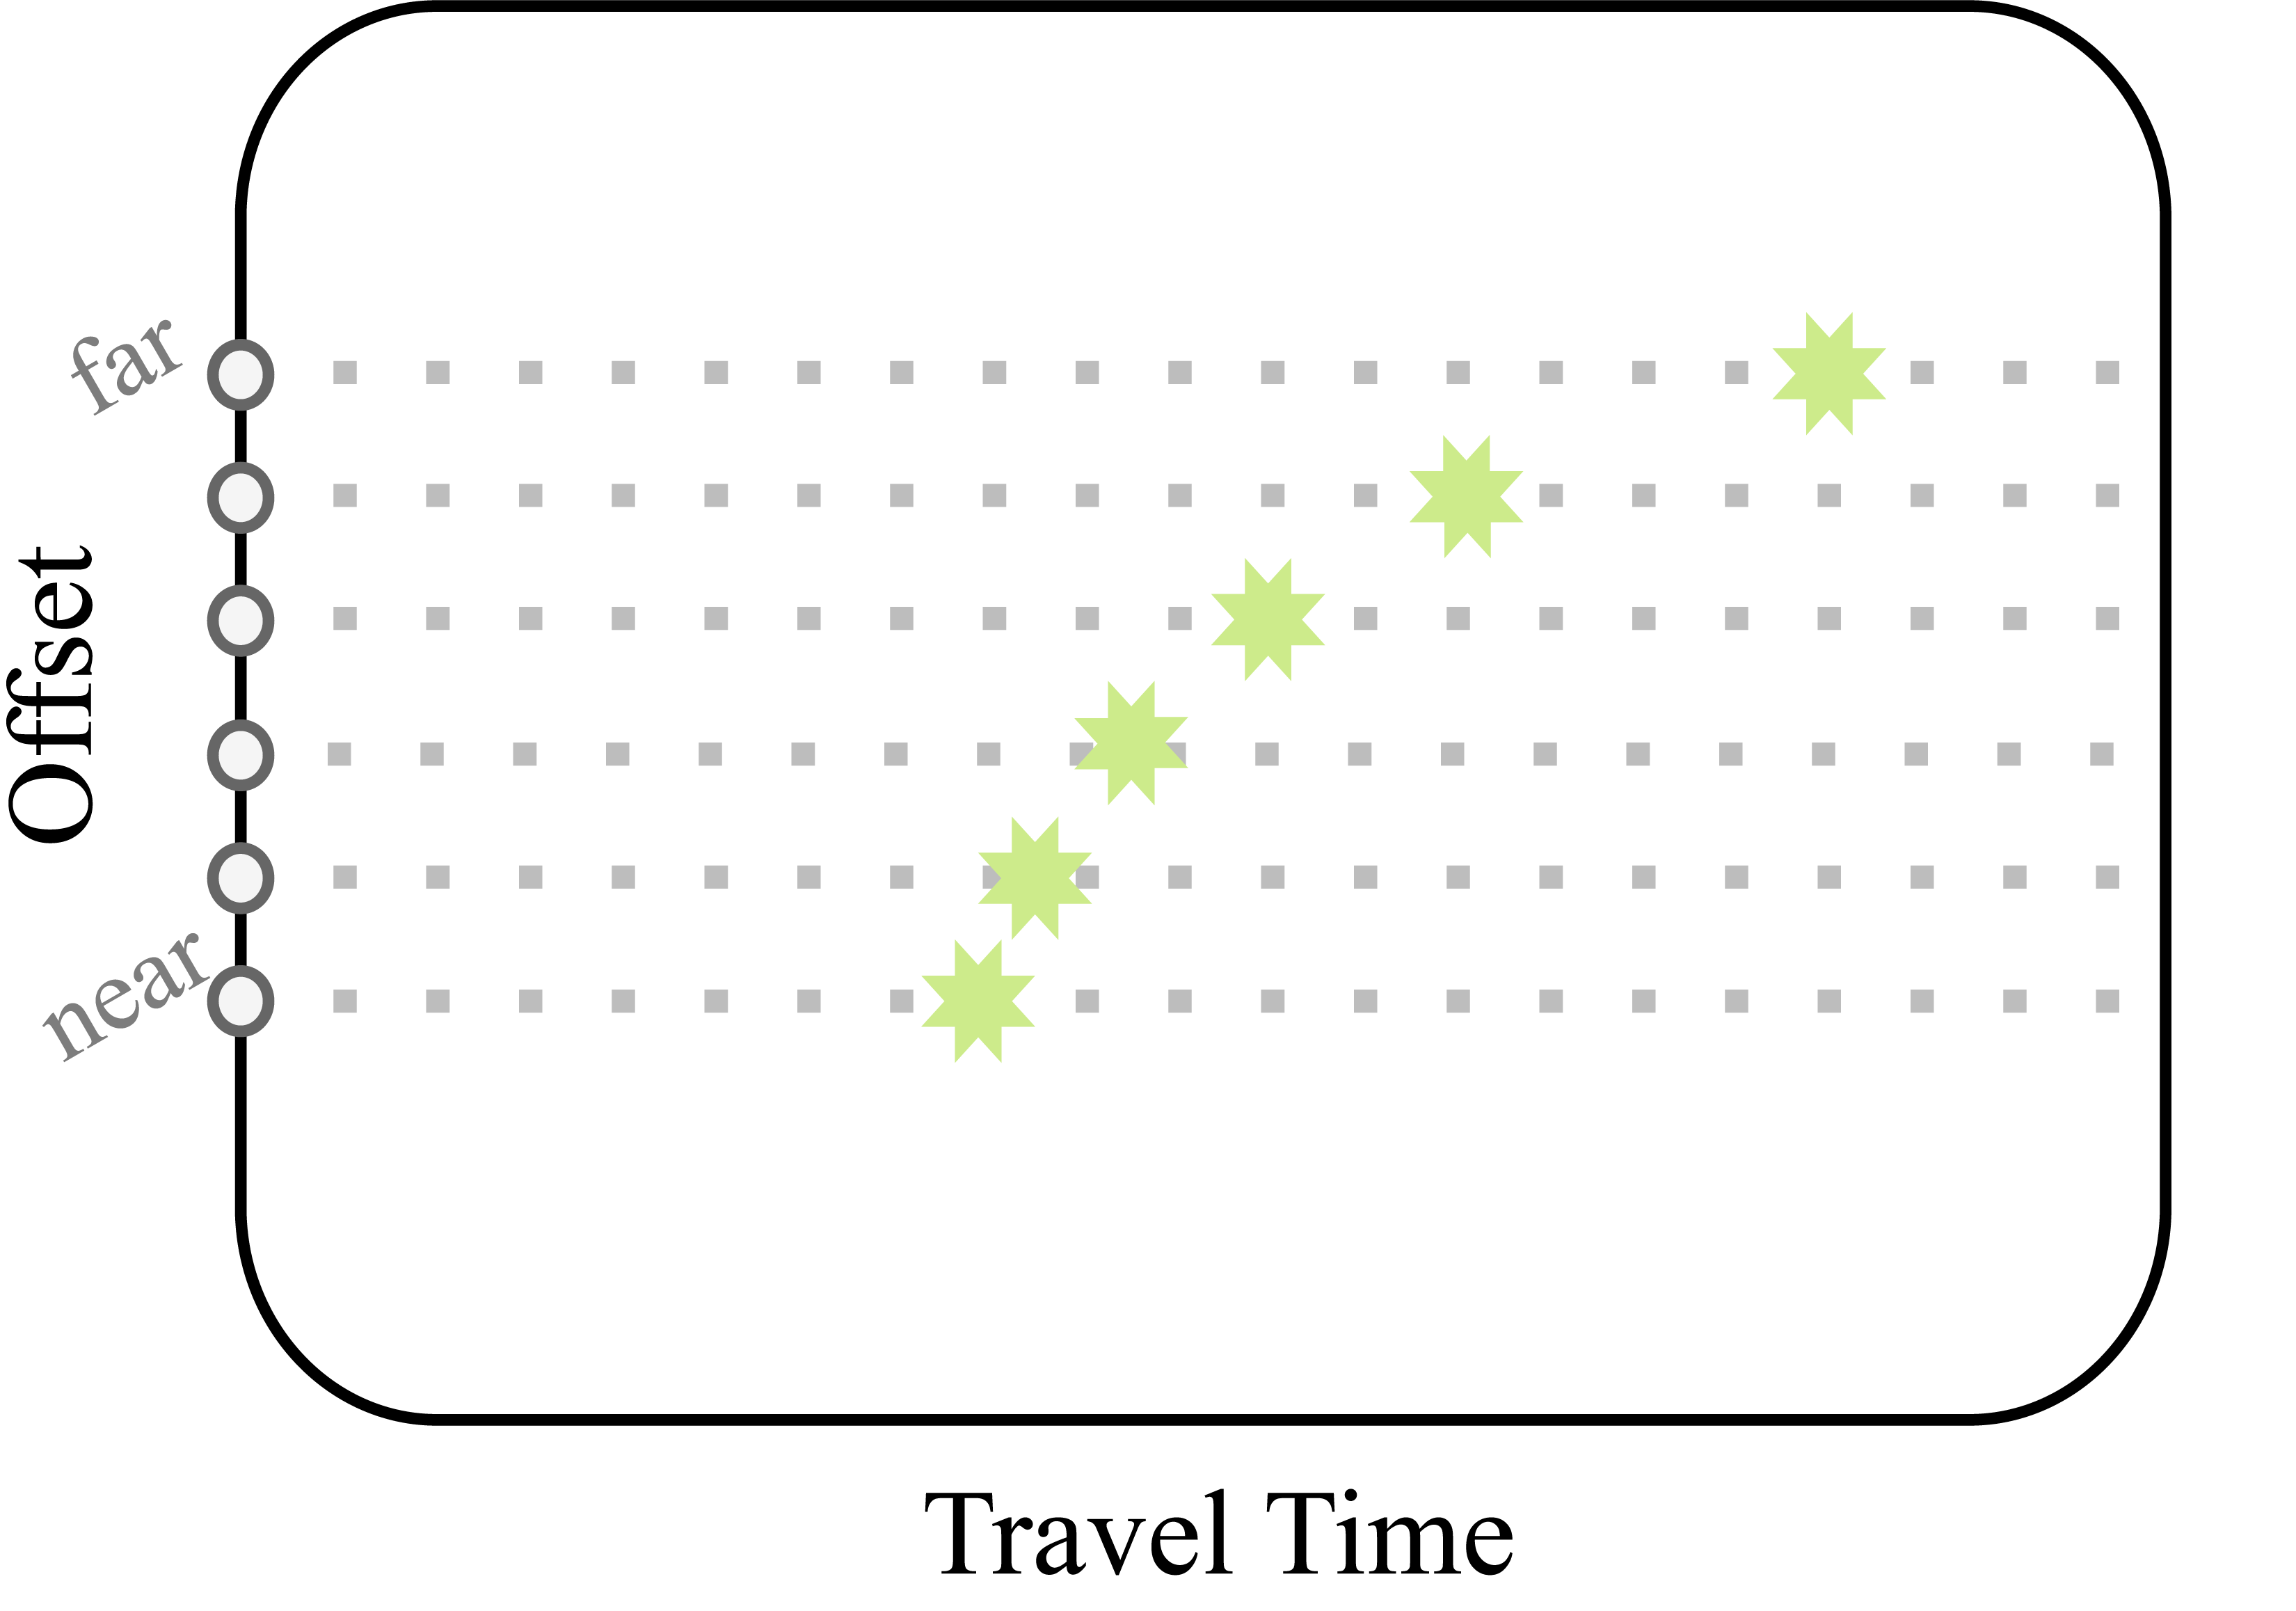
\includegraphics[height=4cm]{04_偏移距与旅行时图像_NMO前.png}
        }\ 
        \subfigure[NMO后旅行时与偏移距的关系]{
            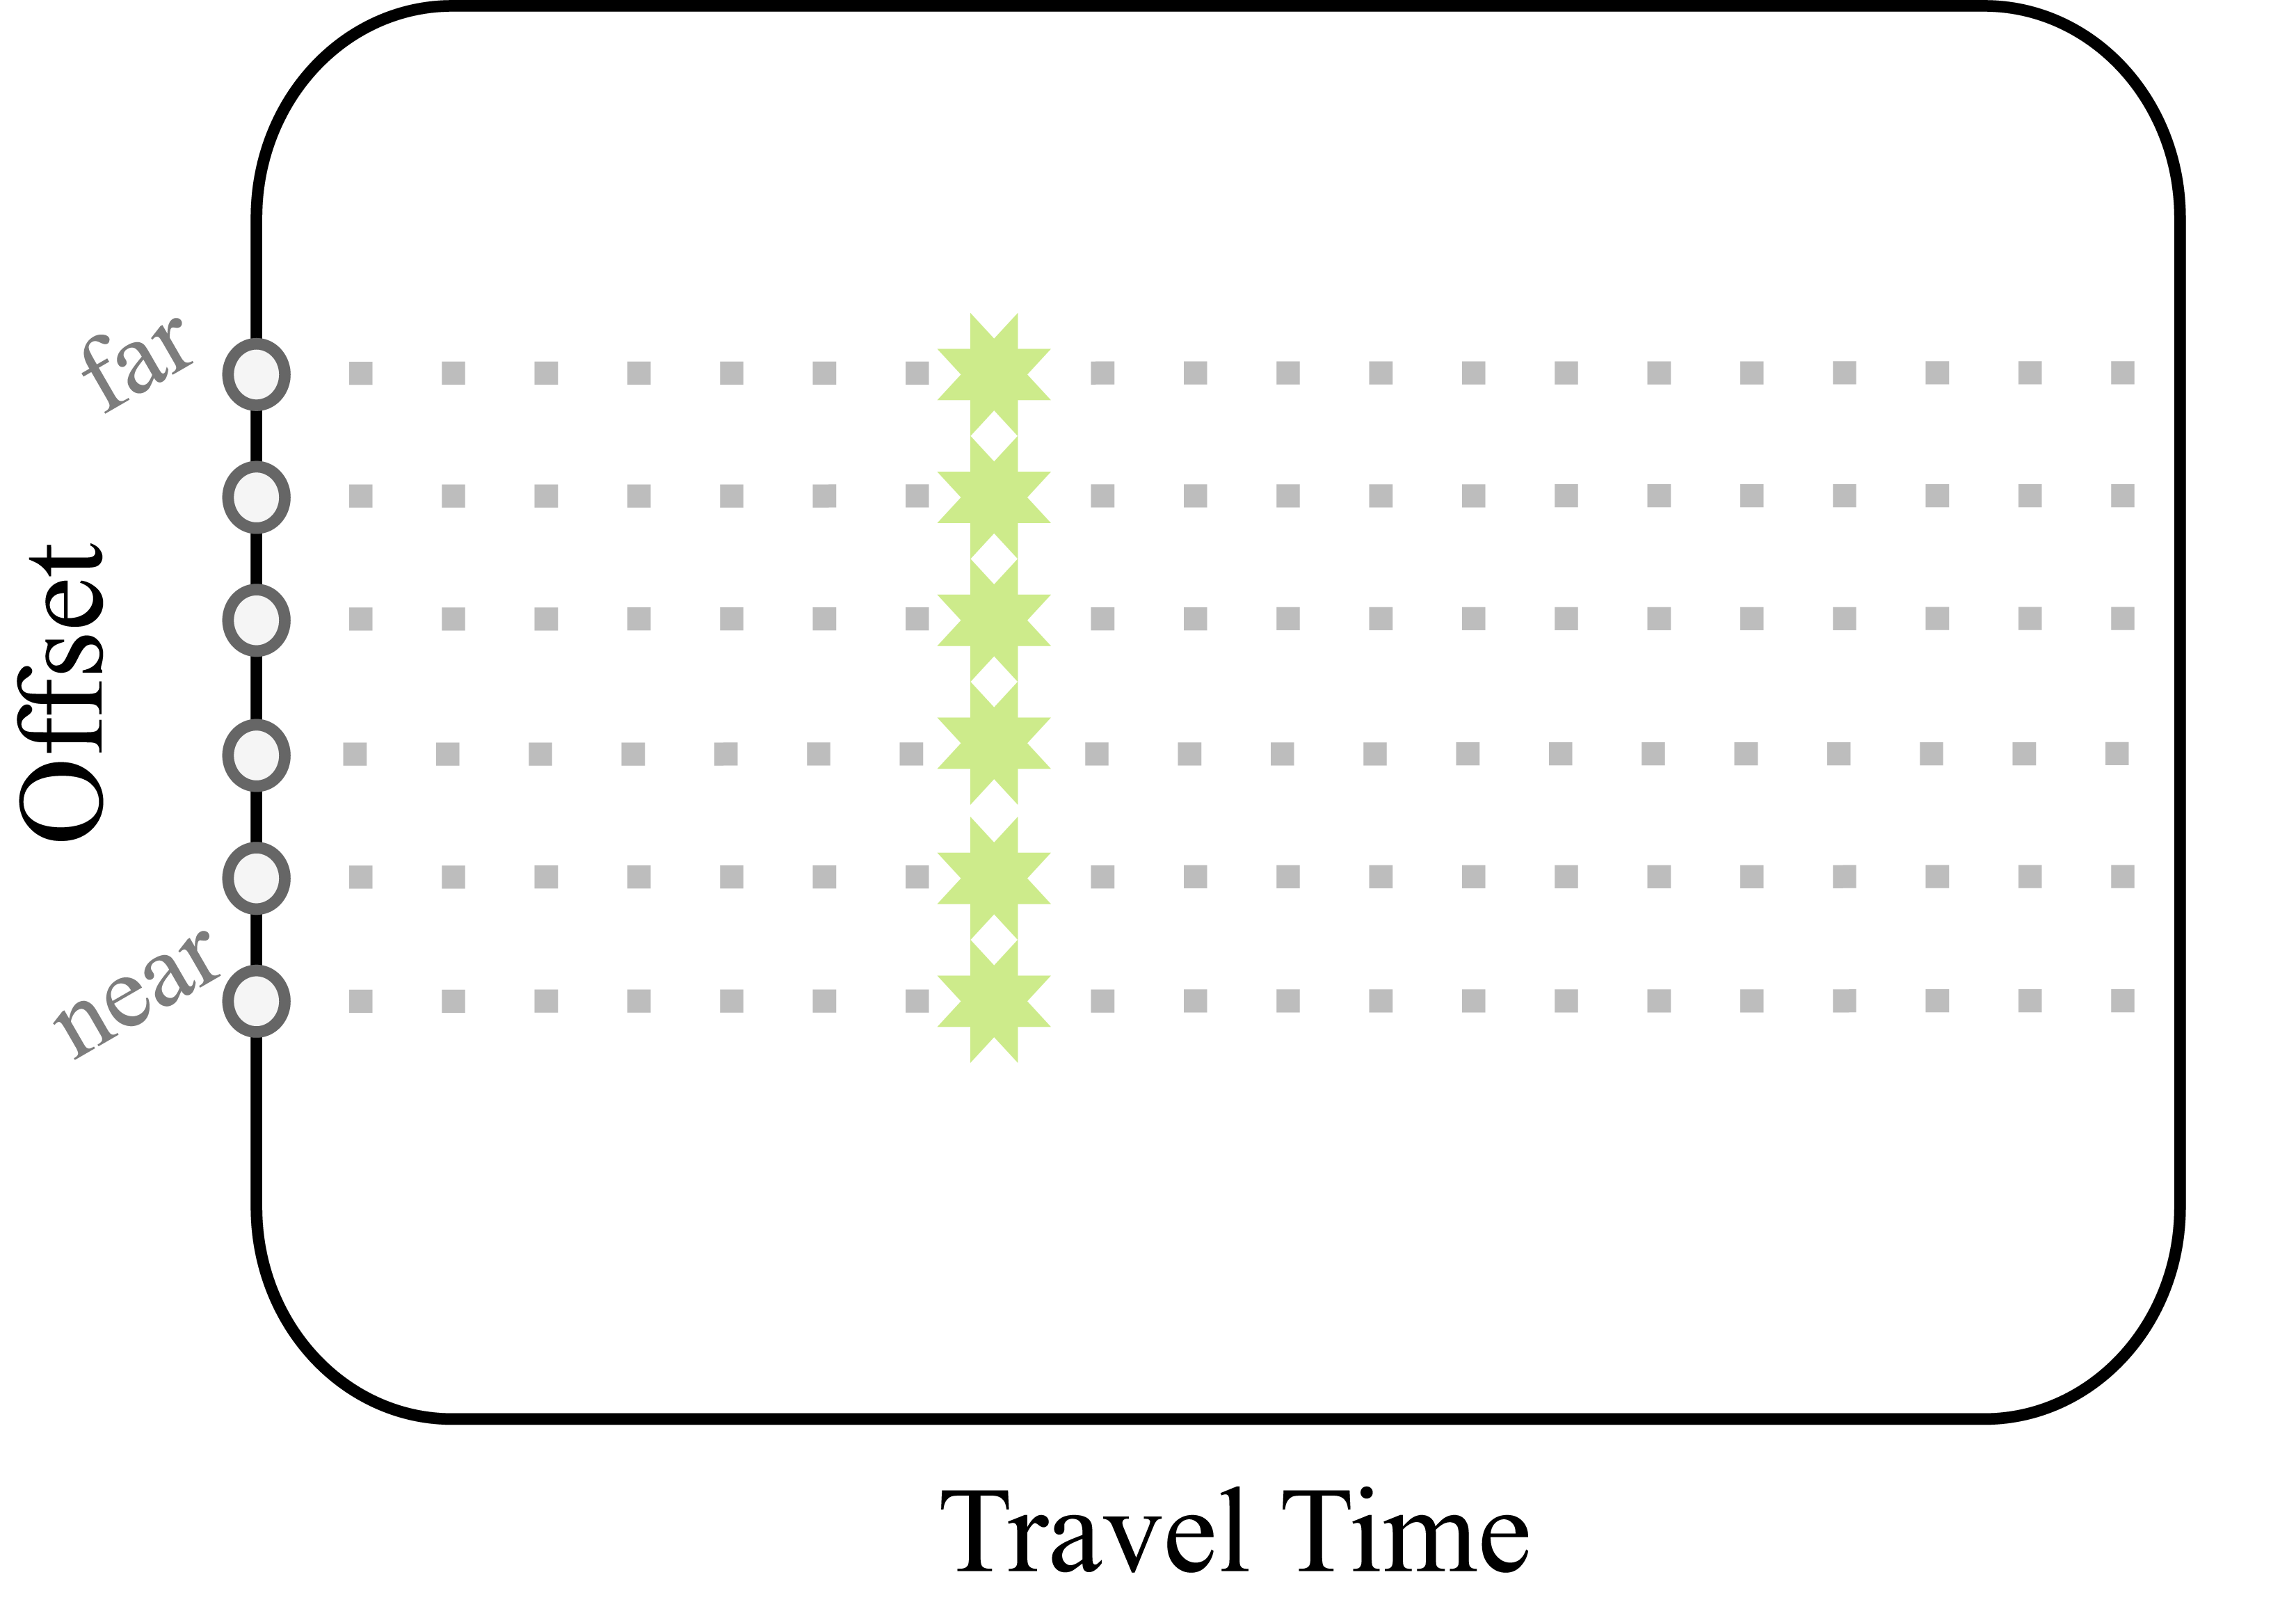
\includegraphics[height=4cm]{05_偏移距与旅行时图像_NMO后.png}
        }
    \end{figure}
\end{frame}

\begin{frame}{速度的选取}
    \begin{figure}[ht]
        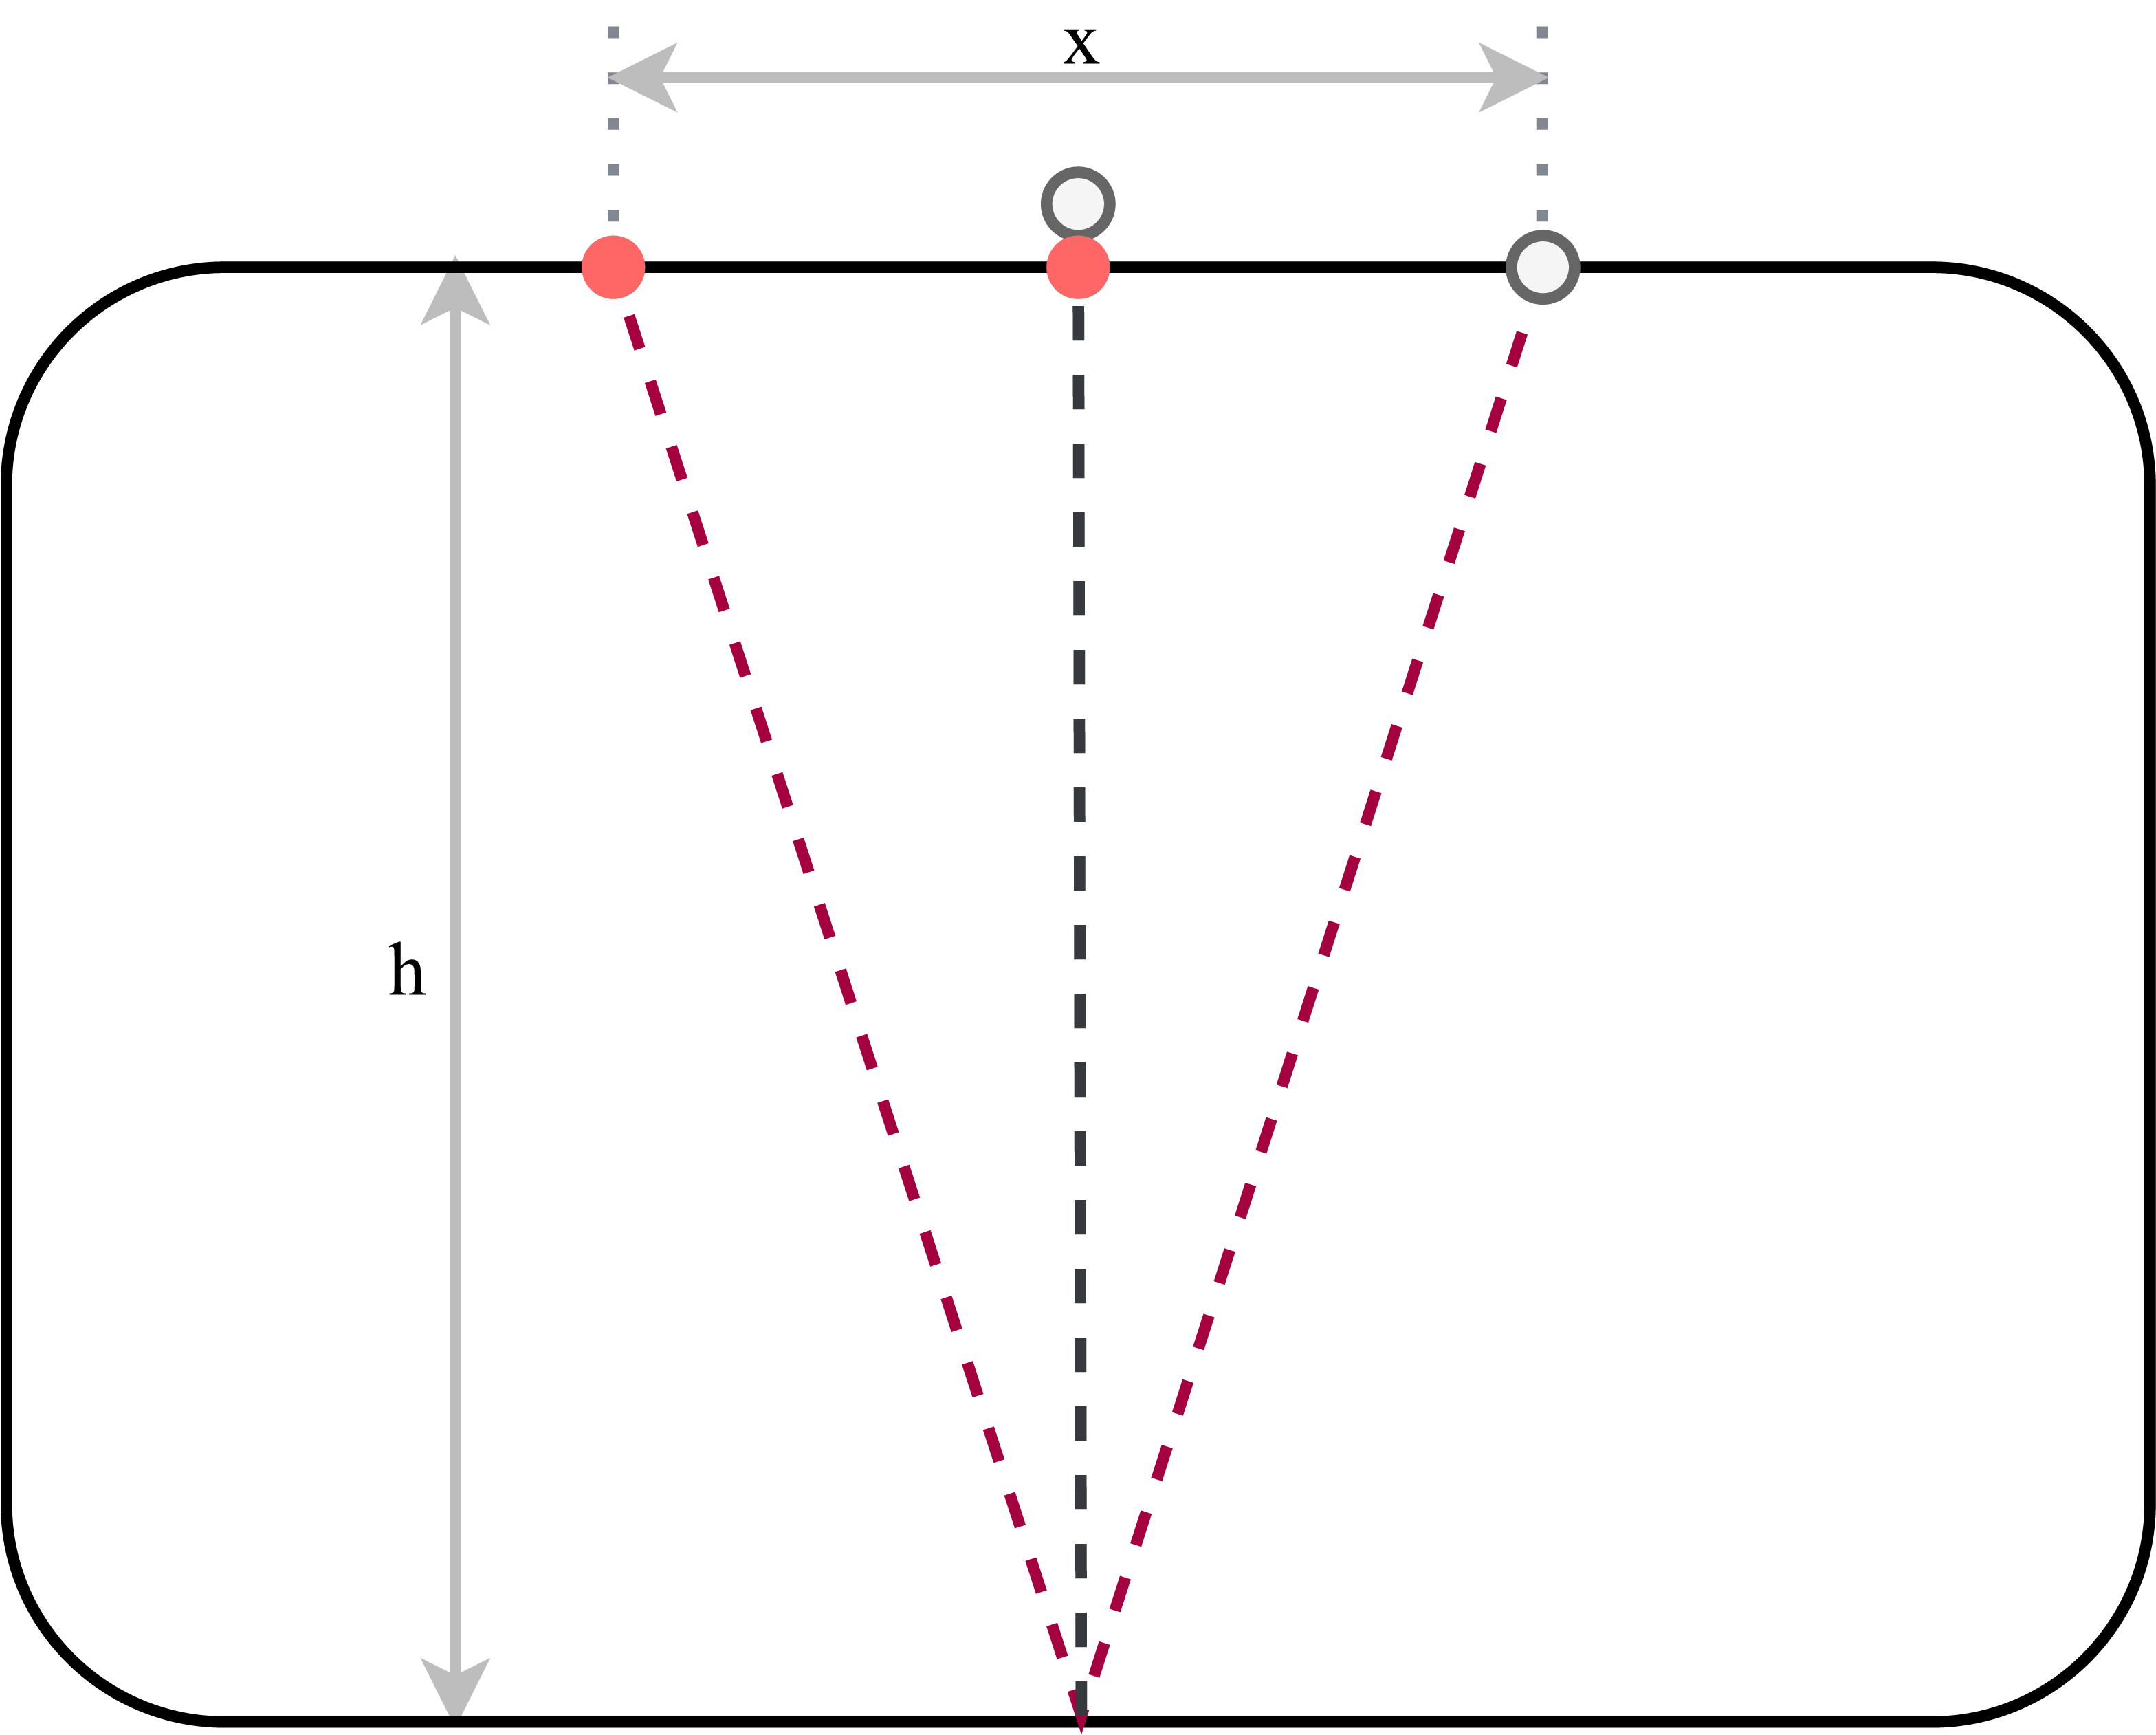
\includegraphics[height=3.5cm]{06_旅行时计算公式.png}
    \end{figure}
    校正后的旅行时$t_0$, 原旅行时$t$, 偏移距$x$, 波速$v$间的关系满足: 
    \[ t_0^2=t^2-\frac{x^2}{v^2} \]
\end{frame}

\begin{frame}{速度的选取}
    \citeauthor{Toldi1989}验证了速度点对应速度谱上的能量峰, 因此对速度点的选择可以转化为在速度谱上进行聚类, 从而寻找聚类中心的问题. 

    \fullcite{Toldi1989}
\end{frame}
